\documentclass[tikz,border=10pt]{standalone}
\begin{document}
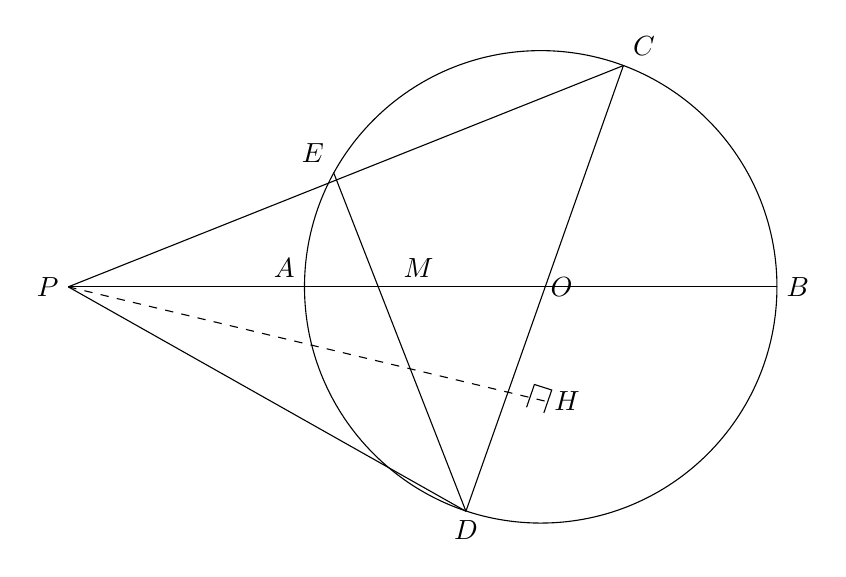
\begin{tikzpicture}[scale=1]

% Coordinates
\coordinate (O) at (0,0);
\coordinate (A) at (-3,0);
\coordinate (B) at (3,0);
\coordinate (P) at (-6,0);
\coordinate (C) at (1.05,2.81);
\coordinate (D) at (-0.95,-2.85);
\coordinate (E) at (-2.63,1.45);
\coordinate (M) at (-1.55,0);
\coordinate (H) at (0.05,-1.45);

% Circle
\draw (O) circle (3);

% Main lines
\draw (P) -- (B);
\draw (P) -- (C);
\draw (P) -- (D);
\draw (E) -- (D);
\draw (D) -- (C);
\draw[dashed] (P) -- (H);

% Right-angle mark at H between CH(=DH line) and PH
\coordinate (R1) at (-0.18,-1.53);
\coordinate (R2) at (-0.08,-1.24);
\coordinate (R3) at (0.14,-1.31);
\coordinate (R4) at (0.04,-1.60);
\draw (R1) -- (R2) -- (R3) -- (R4);

% Labels
\node[left] at (P) {$P$};
\node[above left] at (A) {$A$};
\node[right] at (B) {$B$};
\node[above right] at (C) {$C$};
\node[below] at (D) {$D$};
\node[above left] at (E) {$E$};
\node[above] at (M) {$M$};
\node[right] at (O) {$O$};
\node[right] at (H) {$H$};

\end{tikzpicture}
\end{document}
